\documentclass[tikz]{standalone}
\usepackage{amsthm, amsmath, mathtools, amssymb} % for math commands and math symbols.

\newcommand*\quot[2]{{^{\textstyle #1}\big/_{\textstyle #2}}}
\DeclareMathOperator{\im}{im}

\begin{document}

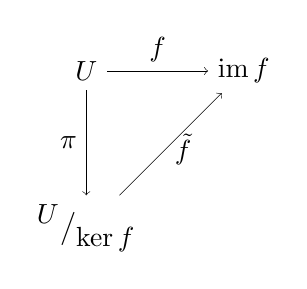
\begin{tikzpicture}
    %%% NODES
    \path (0,0) node(x) {$U$}
    (2,0) node(y) {$\im f$} (0,-2) node(z) {$\displaystyle\quot{U}{\ker f}$};
    %%% LINES
    \draw[very thin,->] (x) --node[above,midway] {$f$} (y);
    \draw[very thin,->] (z) --node[right,pos=0.45] {$\tilde{f}$} (y);
    \draw[very thin,->] (x) --node[left,midway] {$\pi$} (z);
\end{tikzpicture}

\end{document}